
\section{Mô hình sinh cử chỉ}

\begin{frame}{Diffusion cho bài toán sinh cử chỉ}
	\textbf{Điểm giống}
	\begin{itemize}
		\item Diffusion \cite{yang2023diffusestylegesture} trên cử chỉ $\bx^{1:M \times D}$ (như width và height trong ảnh).
		\begin{itemize}
			\item $M$ : frame theo thời gian
			\item $D=1141$ : đặc trưng khung xương của từng khung hình
		\end{itemize}
		\item Classifier-Free Diffusion với $\bx_0$ objective. Latent vector $256$.
		\end{itemize}
		
		\pause
		\textbf{Điểm khác}
		
		\begin{itemize}
			\item Sinh có điều kiện:
			\begin{itemize}
				\item Điều kiện cảm xúc: $c = \big[ \mathbf{s}, \mathbf{e}, \mathbf{a}, \mathbf{v} \big]$ và $c_{\varnothing} = \big[ \varnothing, \varnothing, \mathbf{a}, \mathbf{v}\big]$.
				\item Nội suy trạng thái giữa hai cảm xúc $\mathbf{e}_1, \mathbf{e}_2$: $c = \big[ \mathbf{s}, \mathbf{e}_1, \mathbf{a}, \mathbf{v} \big]$ và $c_{\varnothing} = \big[ \mathbf{s}, \mathbf{e}_2, \mathbf{a}, \mathbf{v} \big]$.
			\end{itemize}
			\item Self-Attention: Mối liên hệ giữa các cảm xúc, cử chỉ khởi tạo và từng frame (tương tự DALL-E 2 - mối liên hệ giữa văn bản và ảnh).
			\item Concat âm thanh và văn bản (Giống ControlNet)
%			\item Học mối liên hệ giữa điều kiện và các frame bằng Local-Cross Attention
		\end{itemize}
\end{frame}



\begin{frame}{Công đoạn 2: Xử lý đặc trưng}
	%	Sử dụng mô hình Diffusion Classifier-Free Guidance (có điều kiện) với cử chỉ $\bx^{1:M \times D}$ làm $\bx_0$ và điều kiện $c = [{\mathbf{s}, \mathbf{a}, \mathbf{e}}, \mathbf{v}]$. $N = 8$, $M = 80 \sim \text{4 giây}$
	%	\vspace{-15pt}
	%	$N=8$ khung hình đầu làm khởi tạo và $M=80$ khung hình để dự đoán
	
	\begin{figure}
		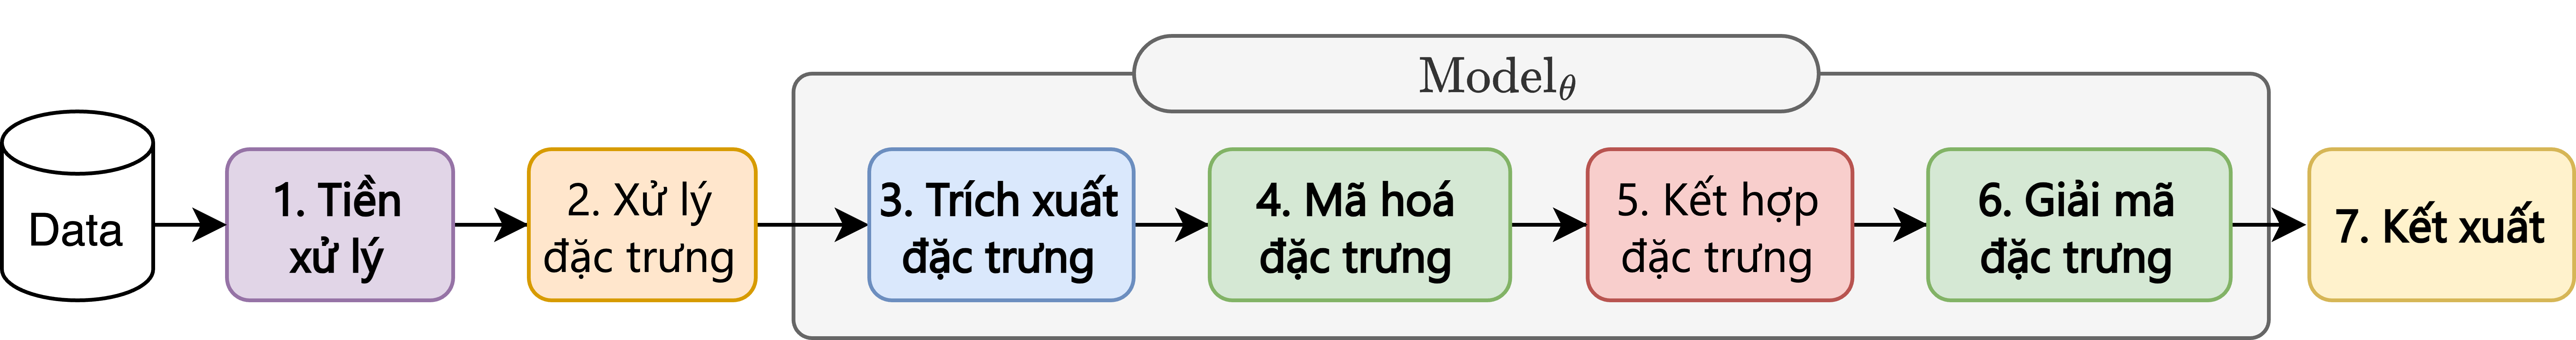
\includegraphics[width=\textwidth]{TotalStage}
	\end{figure}
	%\textbf{Âm thanh}
	
	%Cử chỉ được chuẩn hoá $\mu( \mathbf{g}) = 0$ và $\sigma = 1$. $\bx_{i} = \frac{\bx_{i} - \mu}{\sigma}$.
	\begin{itemize}
		\item \textbf{Cử chỉ}: Chuẩn hoá dữ liệu. $\mathbf{g}^{\operatorname{length}} \xrightarrow{ \text{Cắt thành đoạn} }$ $\mathbf{g}^{[N + M] \times D}$
		\begin{itemize}
			\item Cử chỉ khởi tạo: $\mathbf{s} \in \mathbb{R}^{[1:N] \times D}$
			\item Cử chỉ ground truth: $\mathbf{x} \in \mathbb{R}^{[1:M] \times D}$
		\end{itemize} \pause
		
		\item \textbf{Âm thanh}:  $\mathbf{a}^{\operatorname{length}} \xrightarrow{ \text{Cắt thành đoạn} } \mathbf{a}^{64000} \xrightarrow{\text{WavLM} } $ $\mathbf{a} \in \mathbb{R}^{[1:M] \times 1024}$ \pause
		
		%	16000
		\item \textbf{Cảm xúc}:   Nhãn $\texttt{"Happy"} \rightarrow$ $\mathbf{e} \in \mathbb{R}^{6}$ \pause
		
		\item \textbf{Văn bản}:  $\mathbf{v}^{\operatorname{length}} \xrightarrow{ \text{Cắt theo TextGrid} } \mathbf{v}^{[1:M]} \xrightarrow{ \text{FastText} } $ $\mathbf{v} \in \mathbb{R}^{[1:M] \times 300}$
	\end{itemize}
	
\end{frame}

\begin{frame}{Công đoạn 3. Trích xuất các đặc trưng}
	
	\begin{figure}
		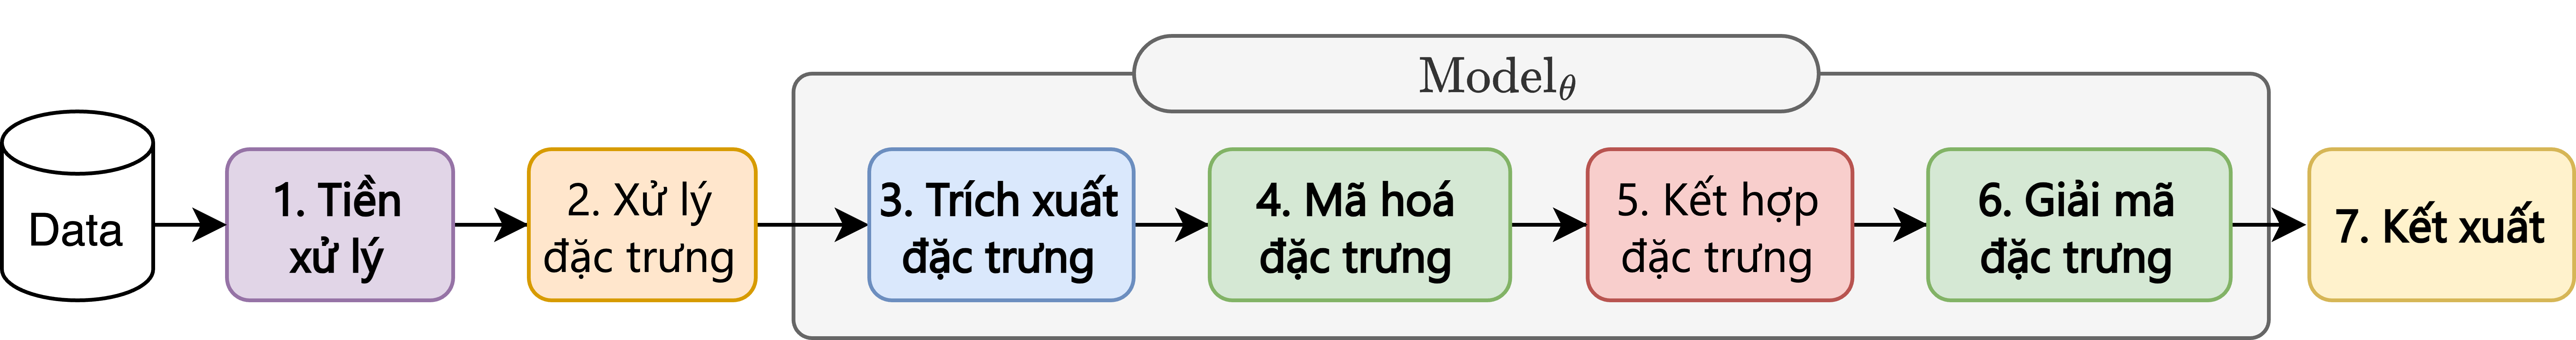
\includegraphics[width=\textwidth]{TotalStage}
	\end{figure}
	\vspace{10pt}
	\begin{itemize}
		\item Âm thanh: $\mathbf{a} \in \mathbb{R}^{ [1:M] \times 1024} \xrightarrow{\text{Linear} } \mathbf{A} \in \mathbb{R}^{[1:M] \times 64}$
		\item Cử chỉ khởi tạo: $\mathbf{s} \in \mathbb{R}^{[1:N] \times D}  \xrightarrow{\text{Linear + Random Mask} } \mathbf{S} \in \mathbb{R}^{192} $ 
		\item Cảm xúc: $\mathbf{e} \in \mathbb{R}^{6}  \xrightarrow{\text{Linear + Random Mask} } \mathbf{E} \in \mathbb{R}^{64} $ 
		\item Văn bản: $\mathbf{v} \in \mathbb{R}^{[1:M] \times 300}  \xrightarrow{\text{Linear} } \mathbf{V} \in \mathbb{R}^{256}$
		\item Timestep: $\mathbf{t} \in \mathbb{R}  \xrightarrow{\text{Linear} } \mathbf{T} \in \mathbb{R}^{256} $ 
		
		
	\end{itemize}
\end{frame}
	
%\begin{frame}{Tổng quan các công đoạn}
%	\begin{figure}
%		\centering
%		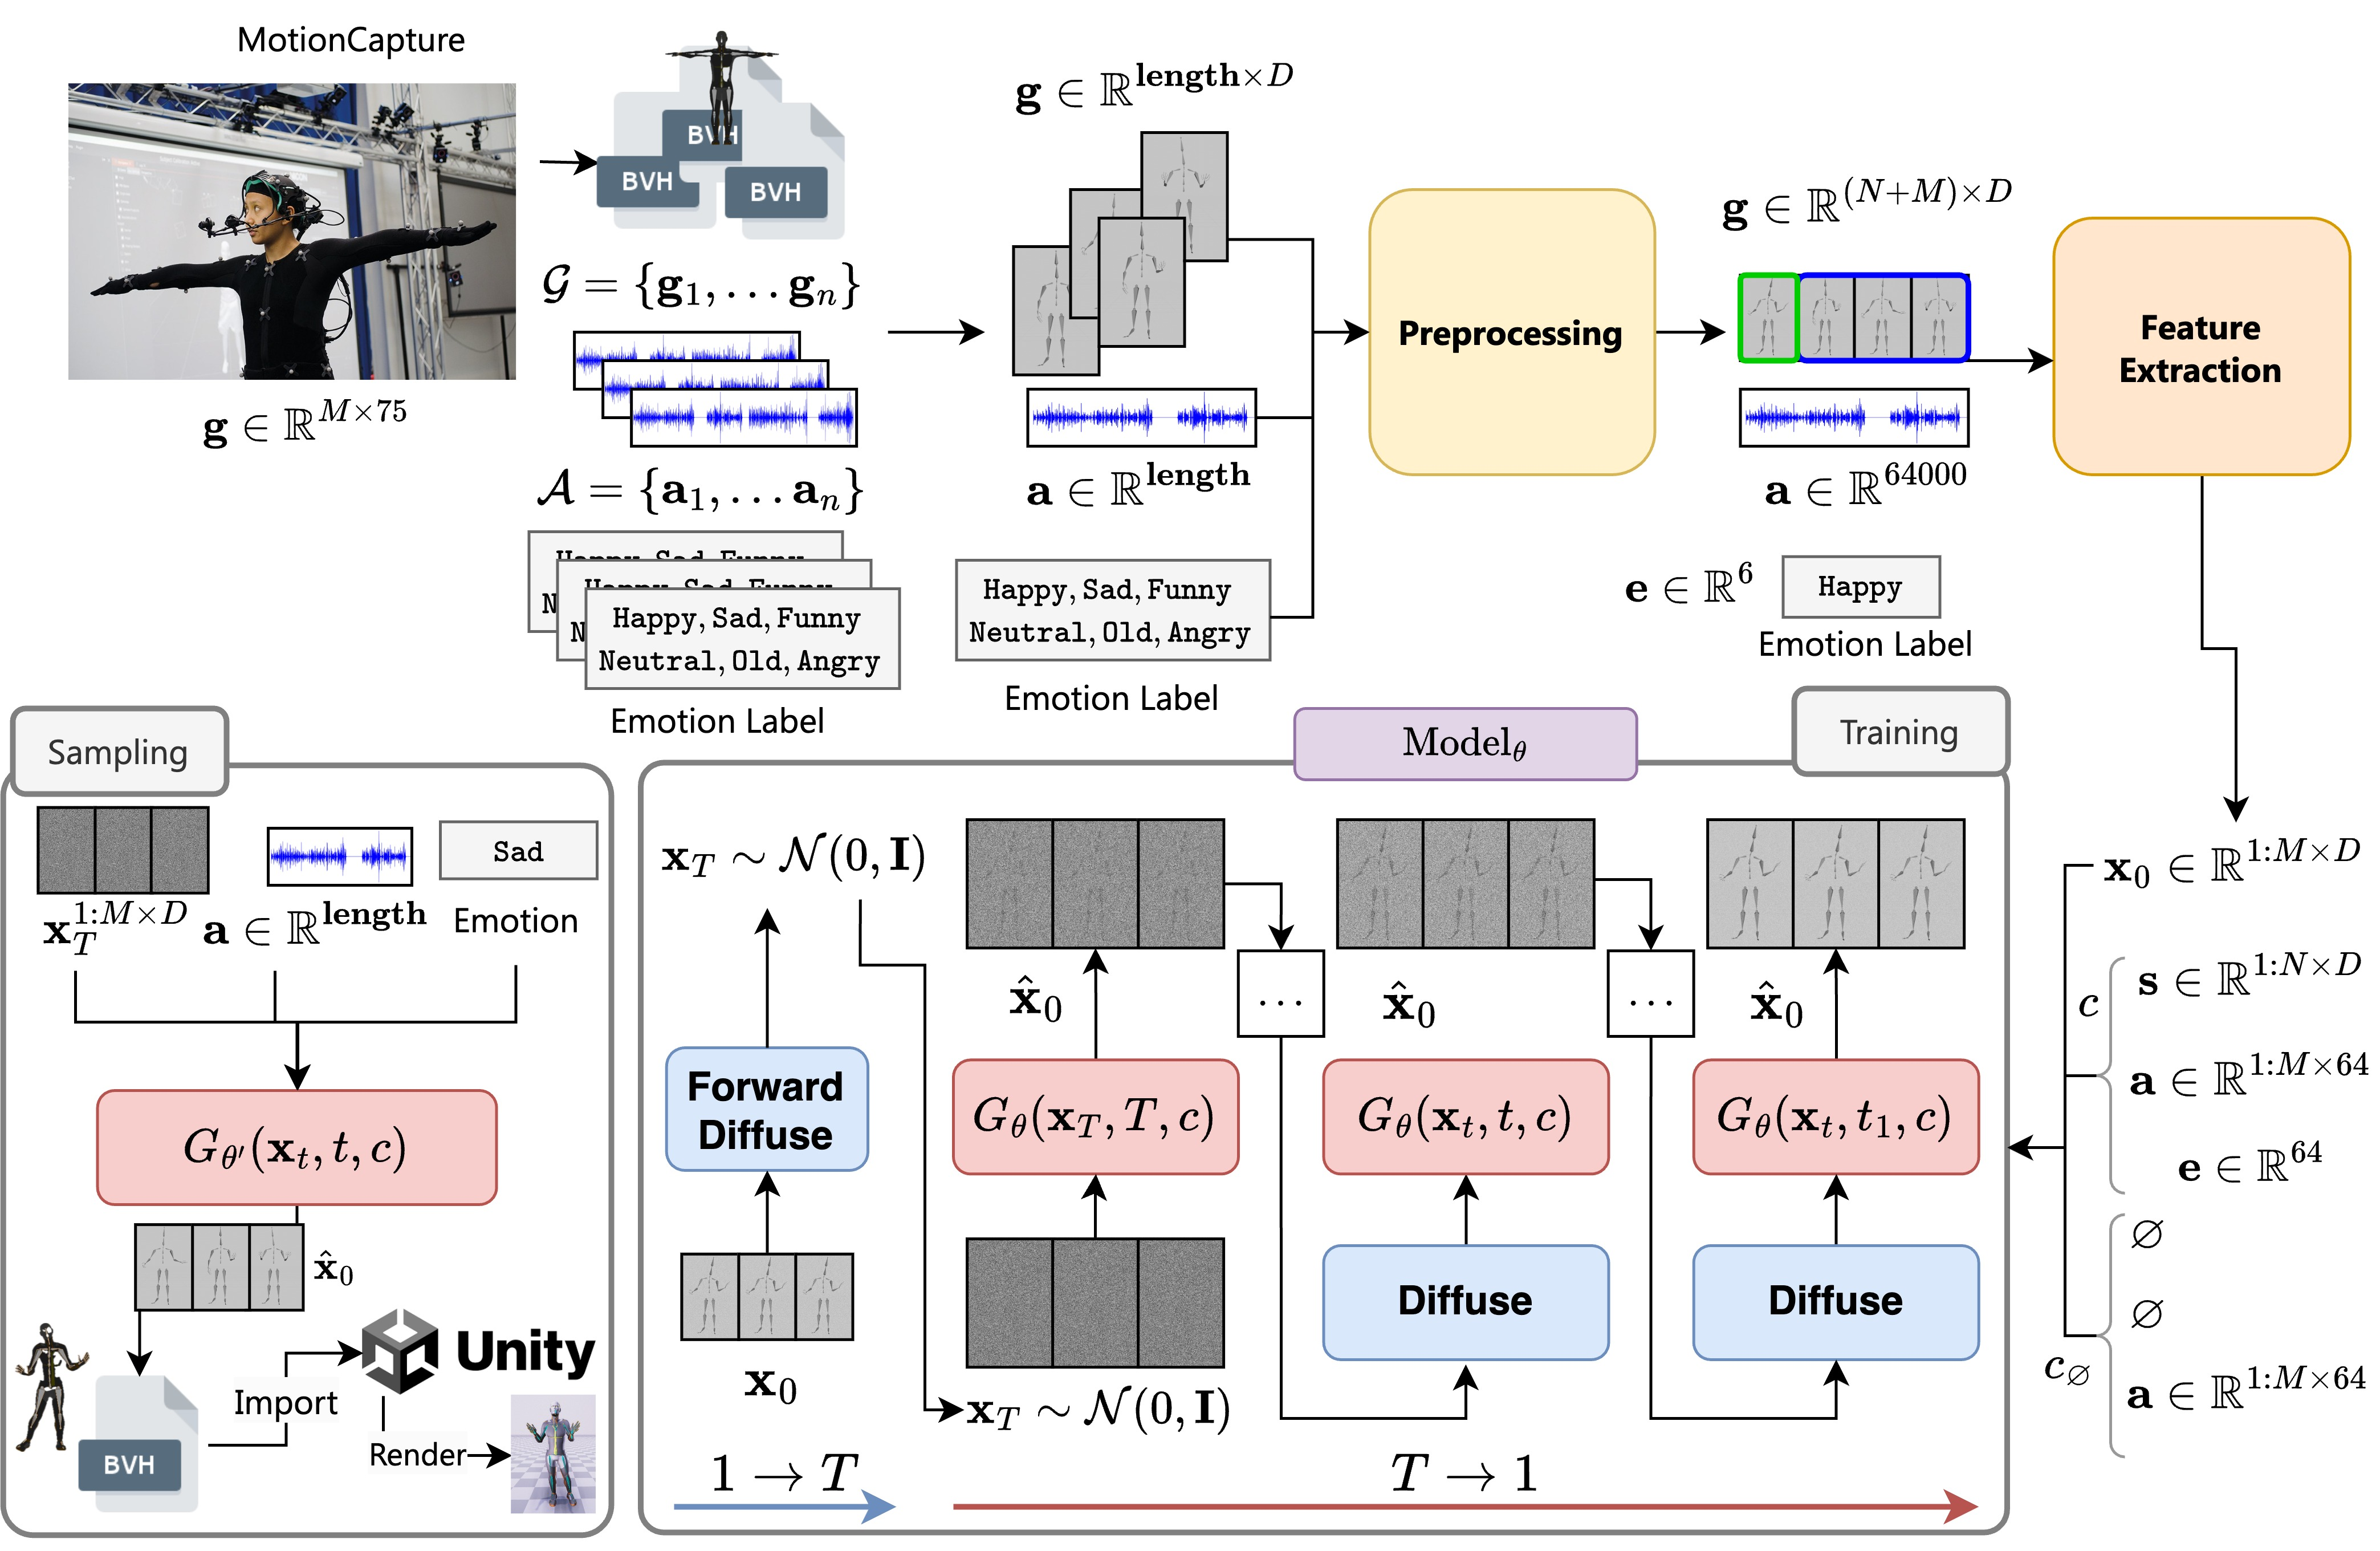
\includegraphics[width=\linewidth]{AllStage}
%	\end{figure}
%	
%\end{frame}

\begin{frame}{Công đoạn 4, 6: Mã hoá và giải mã đặc trưng}
	\begin{figure}
		\centering
		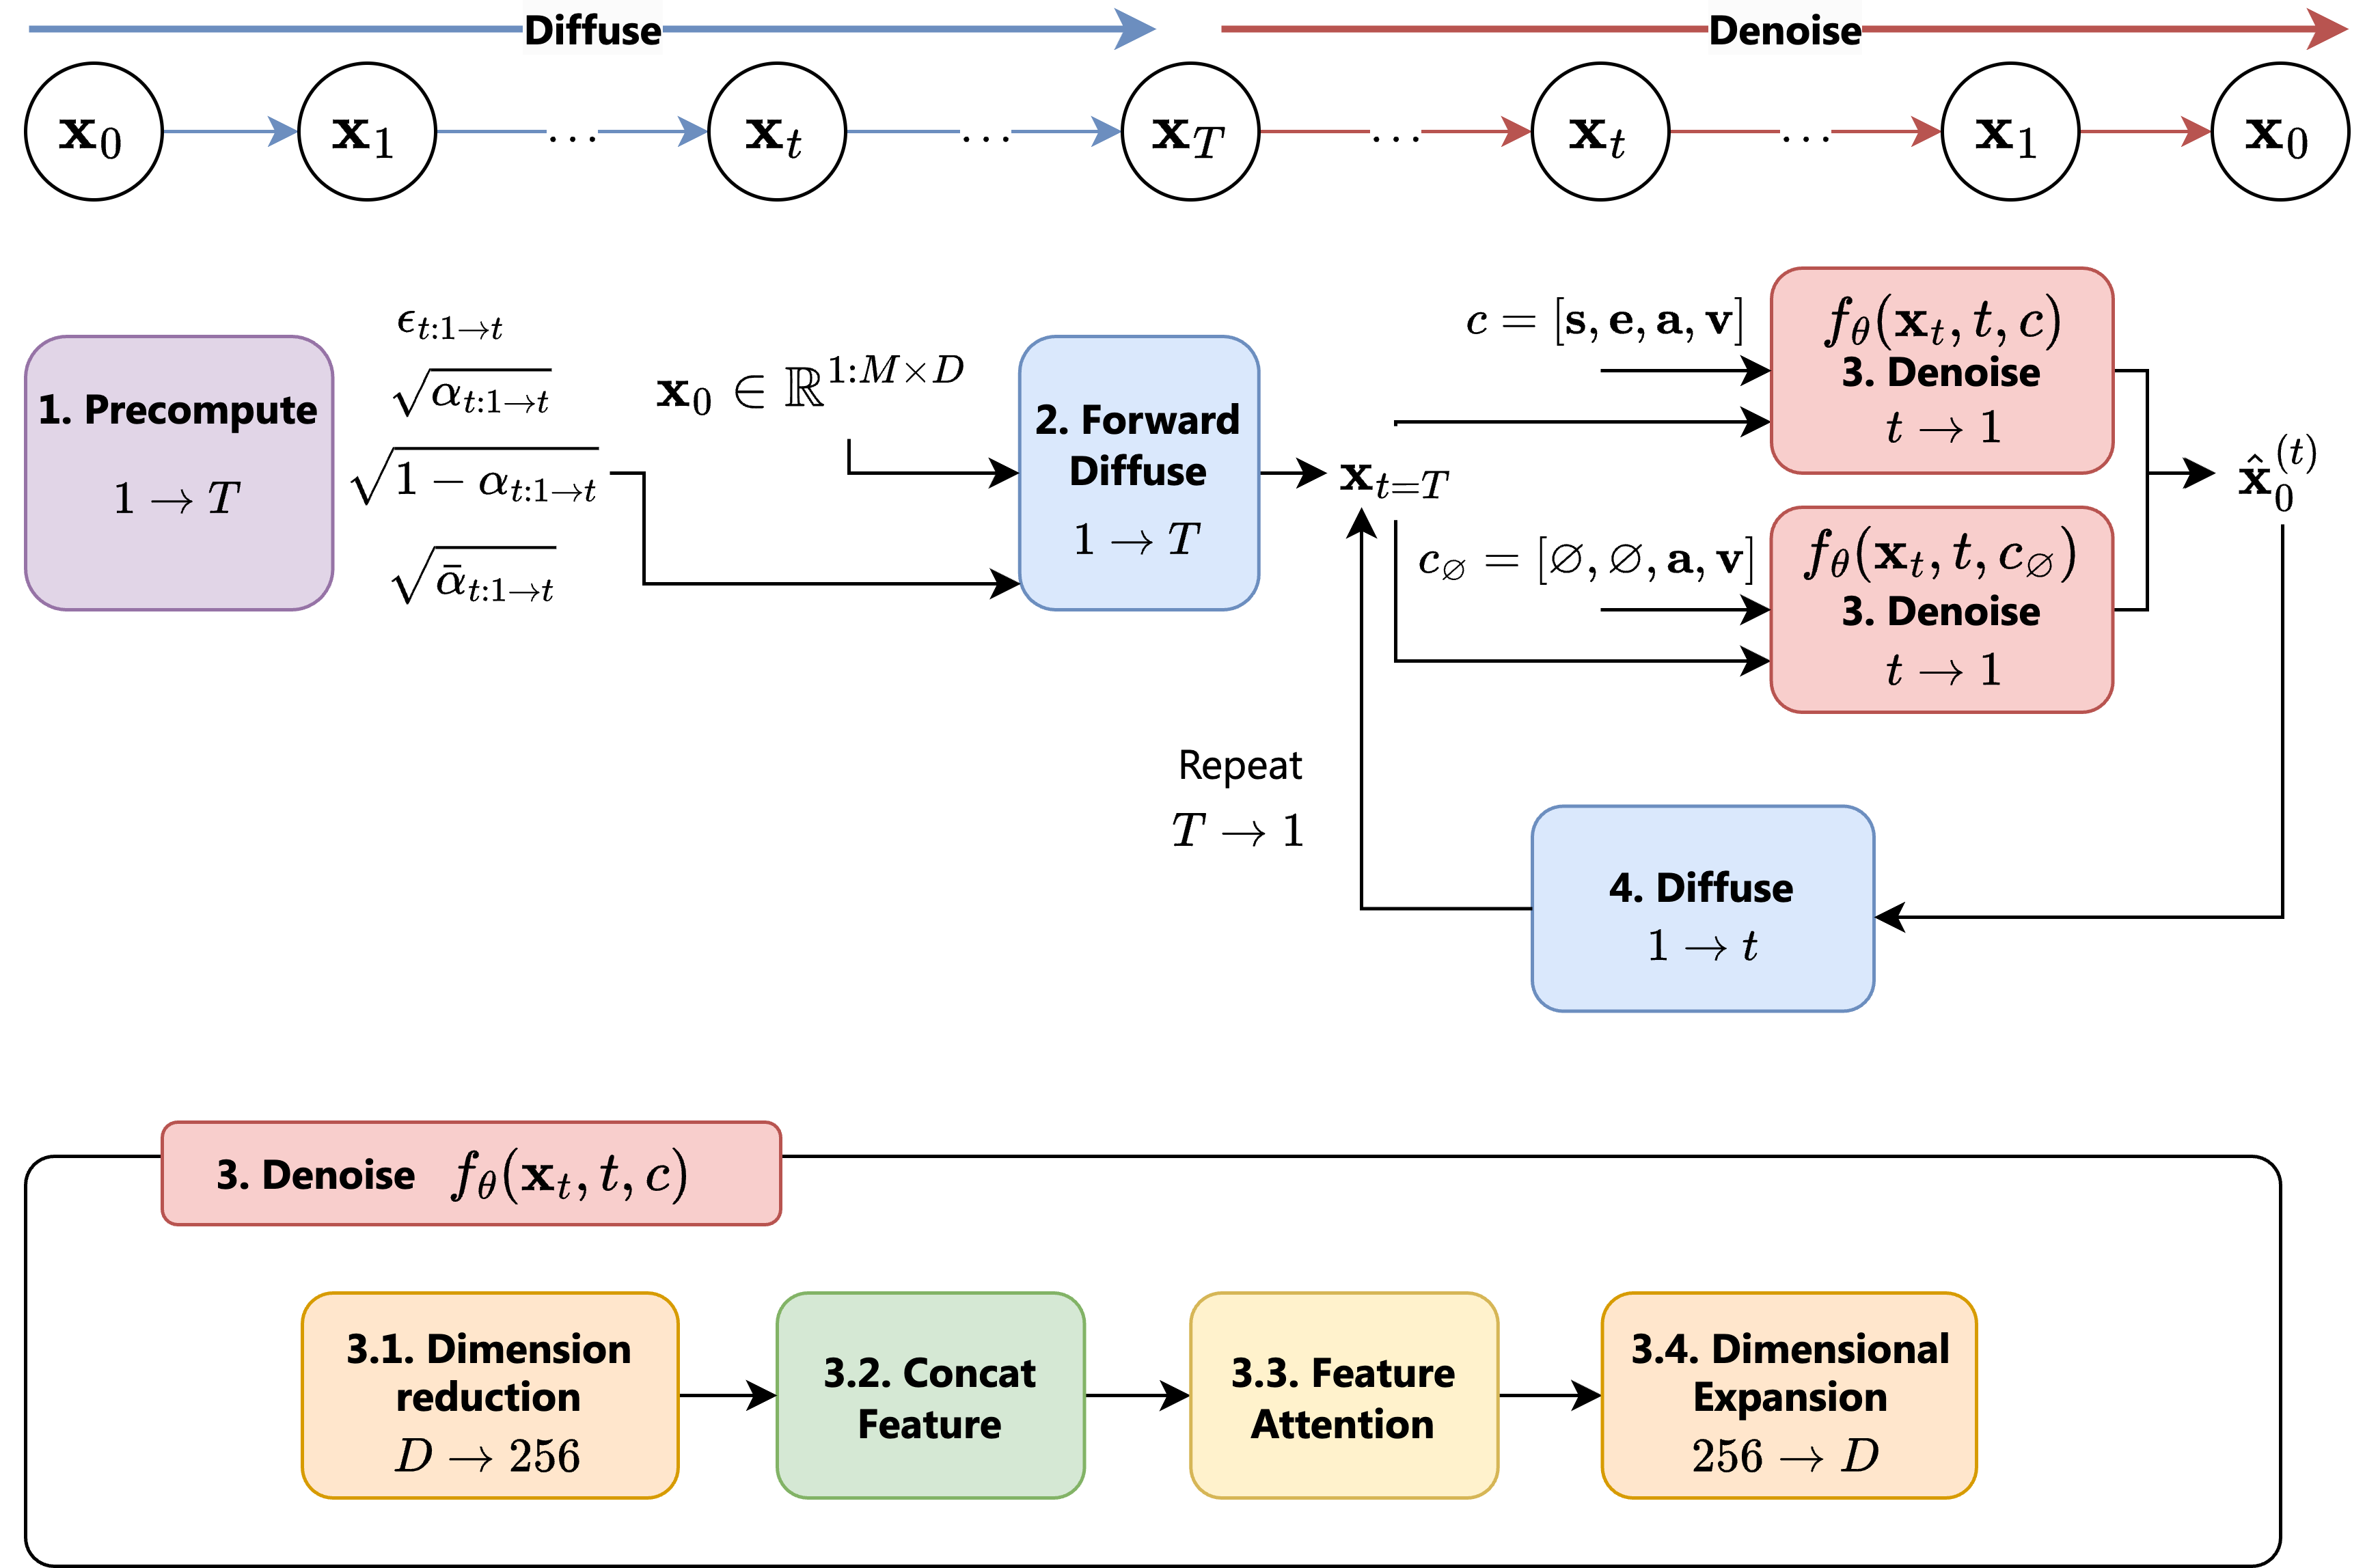
\includegraphics[width=\linewidth]{ModelStage}
	\end{figure}
\end{frame}

%\begin{frame}{Các công đoạn trong mô hình OHGesture}
%	\begin{figure}
%		\centering
%		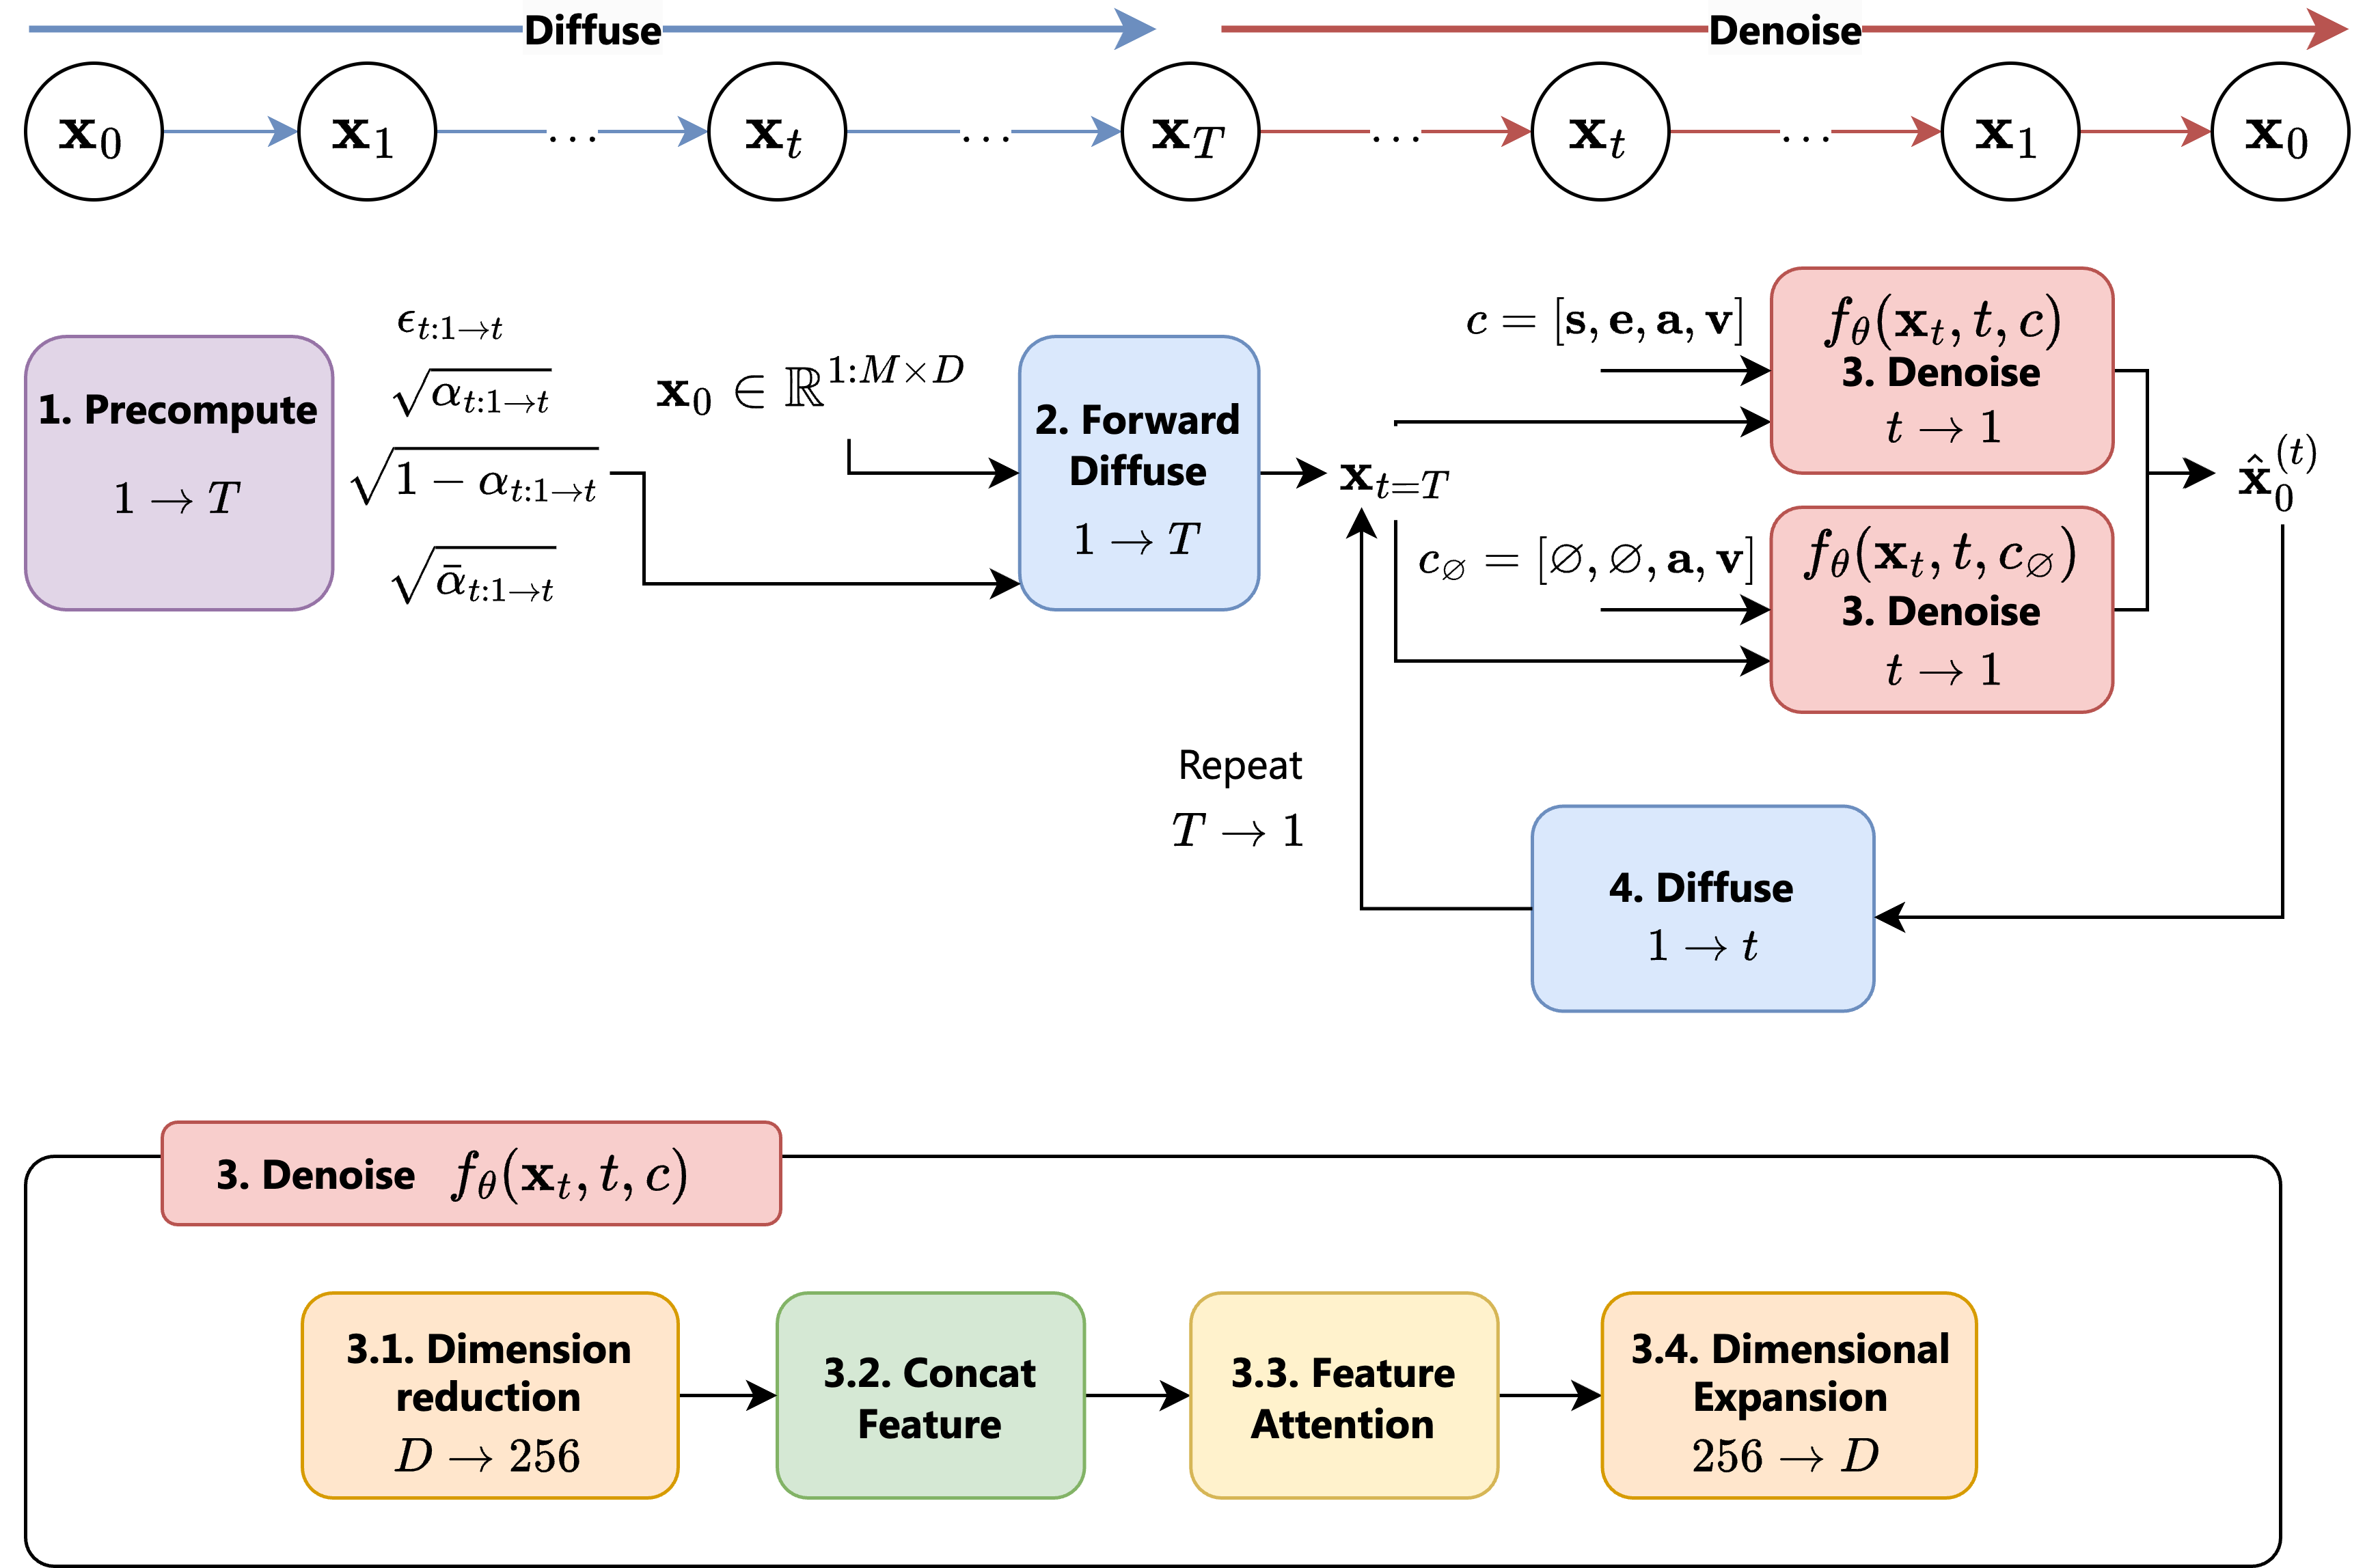
\includegraphics[width=\linewidth]{ModelStage}
%	\end{figure}
%\end{frame}

\begin{frame}{Quá trình học Online và Offline}
	\begin{figure}
		\centering
		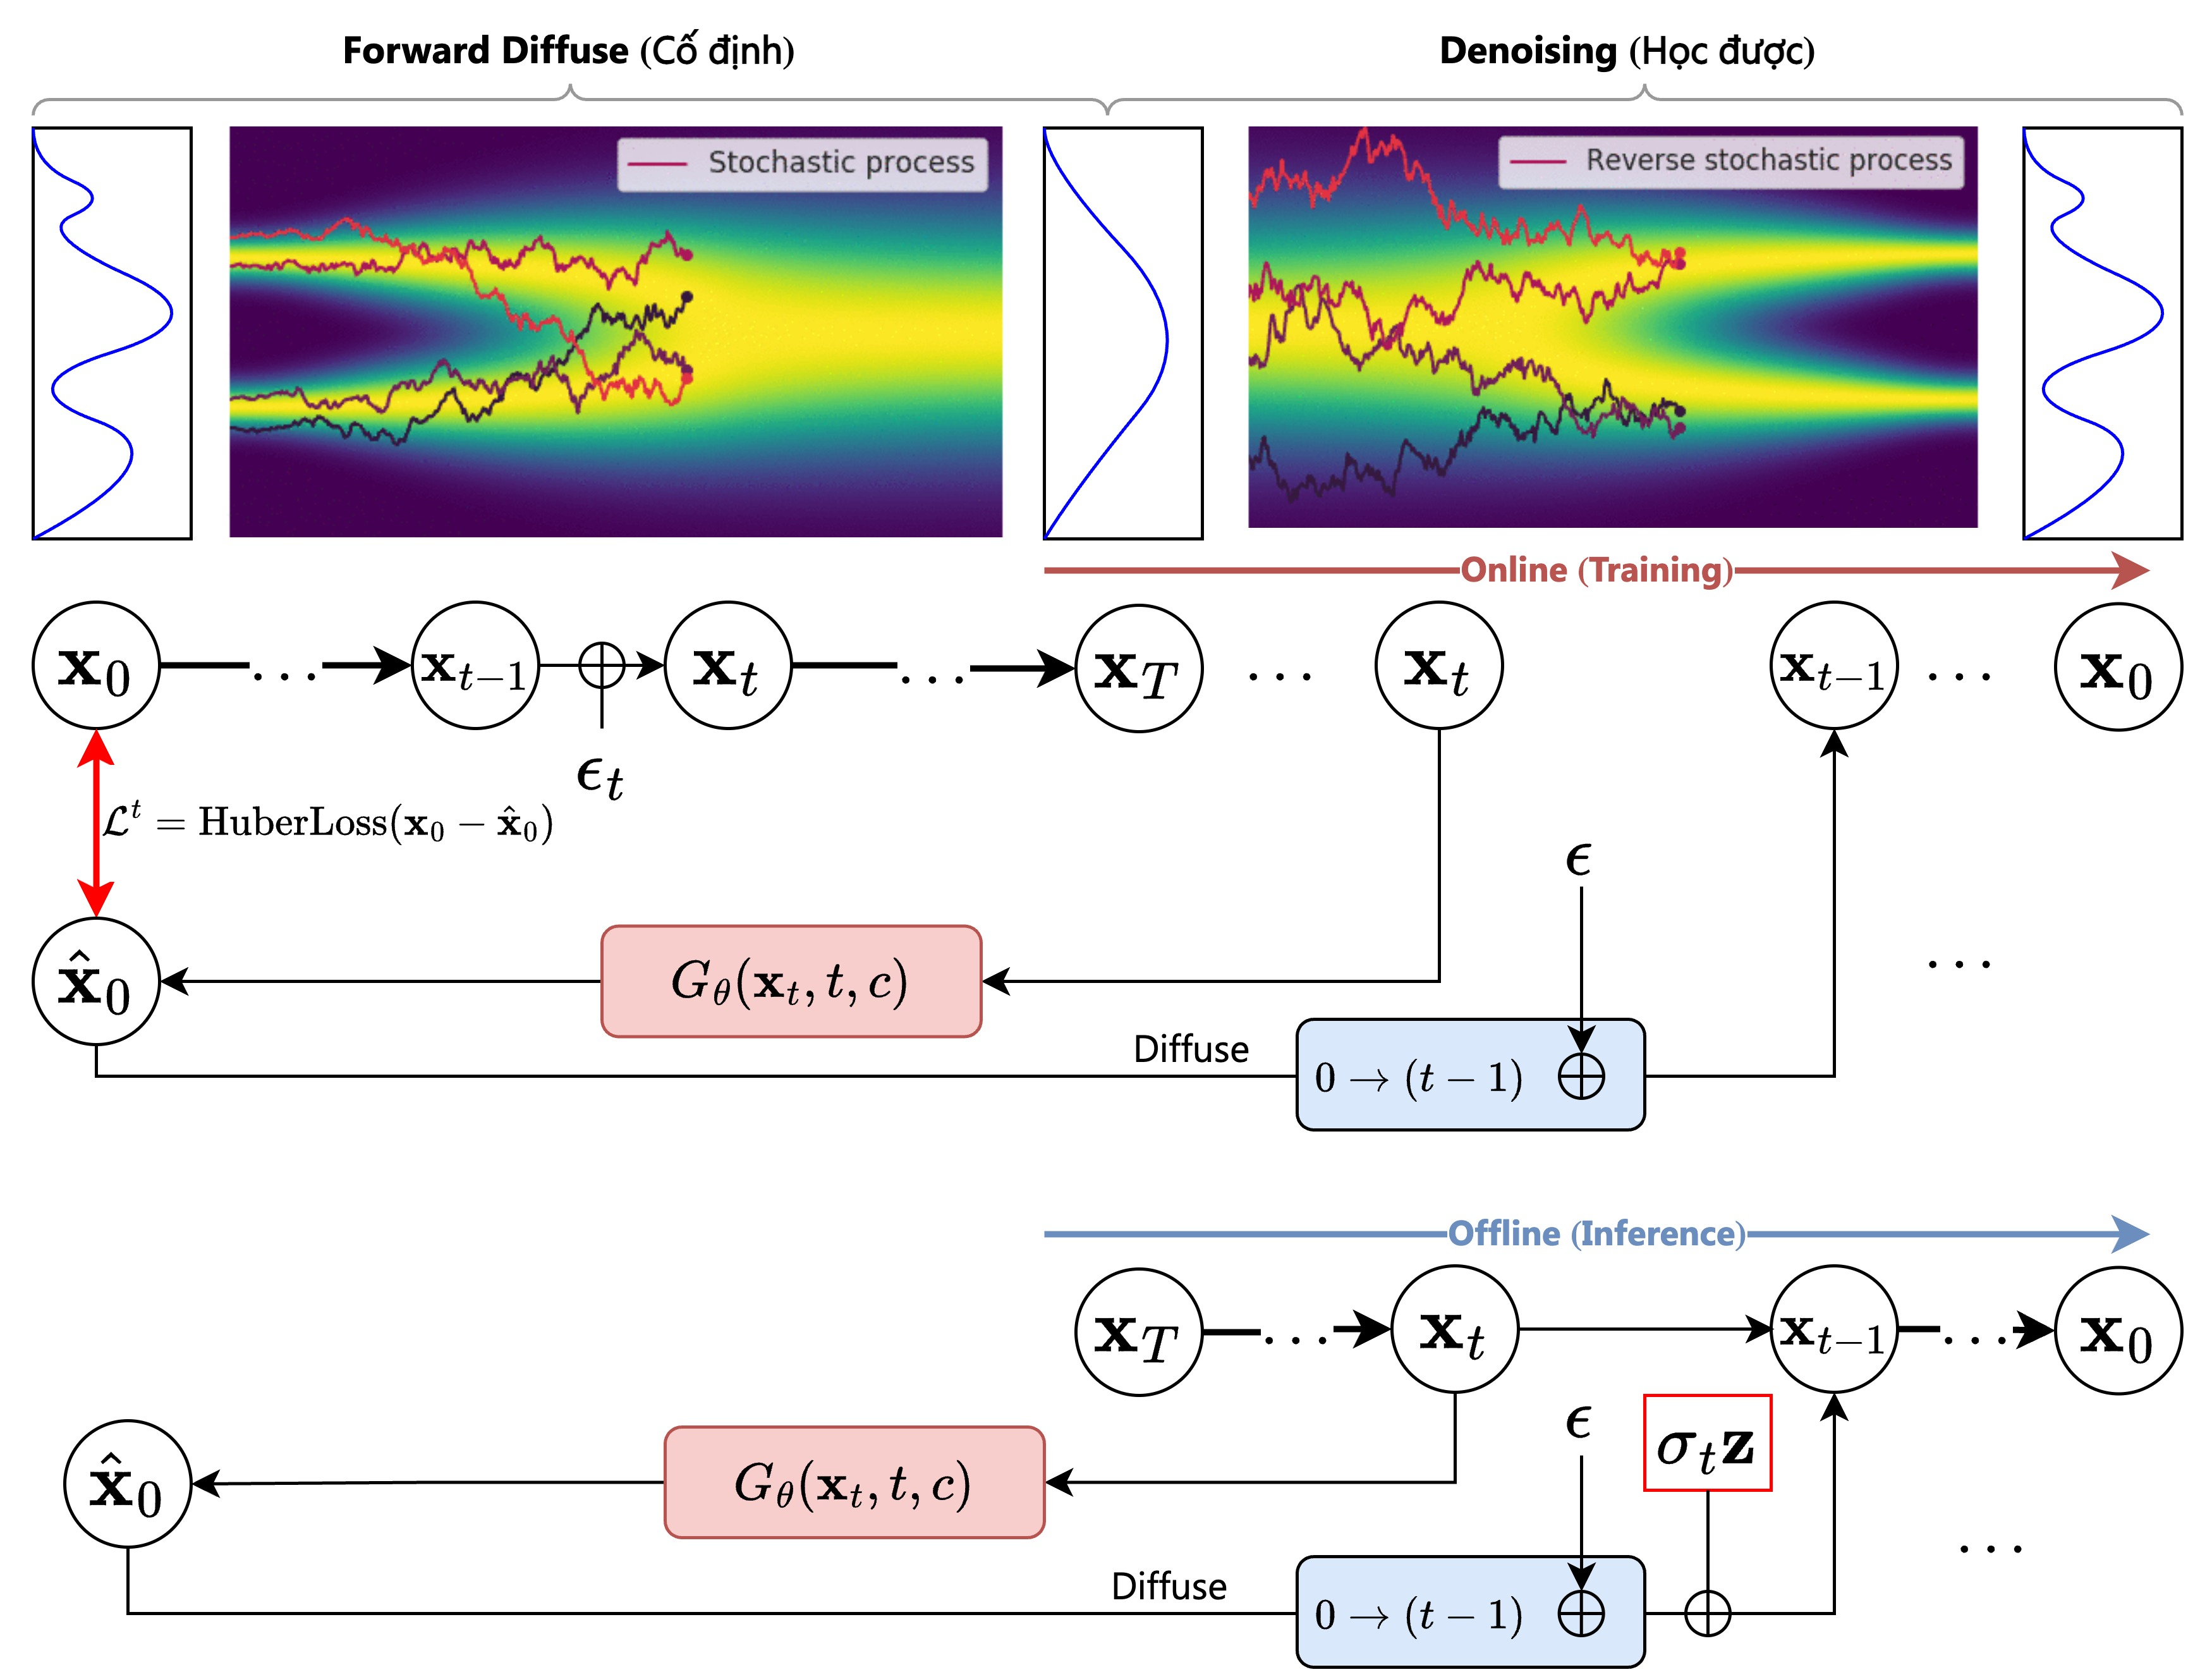
\includegraphics[width=\linewidth]{OnlineAndOffline}
	\end{figure}
\end{frame}


\begin{frame}{Công đoạn 5: Kết hợp các đặc trưng}
%	Cross-Local Attention and Self-Attention
%	\begin{figure}
%		\centering
%		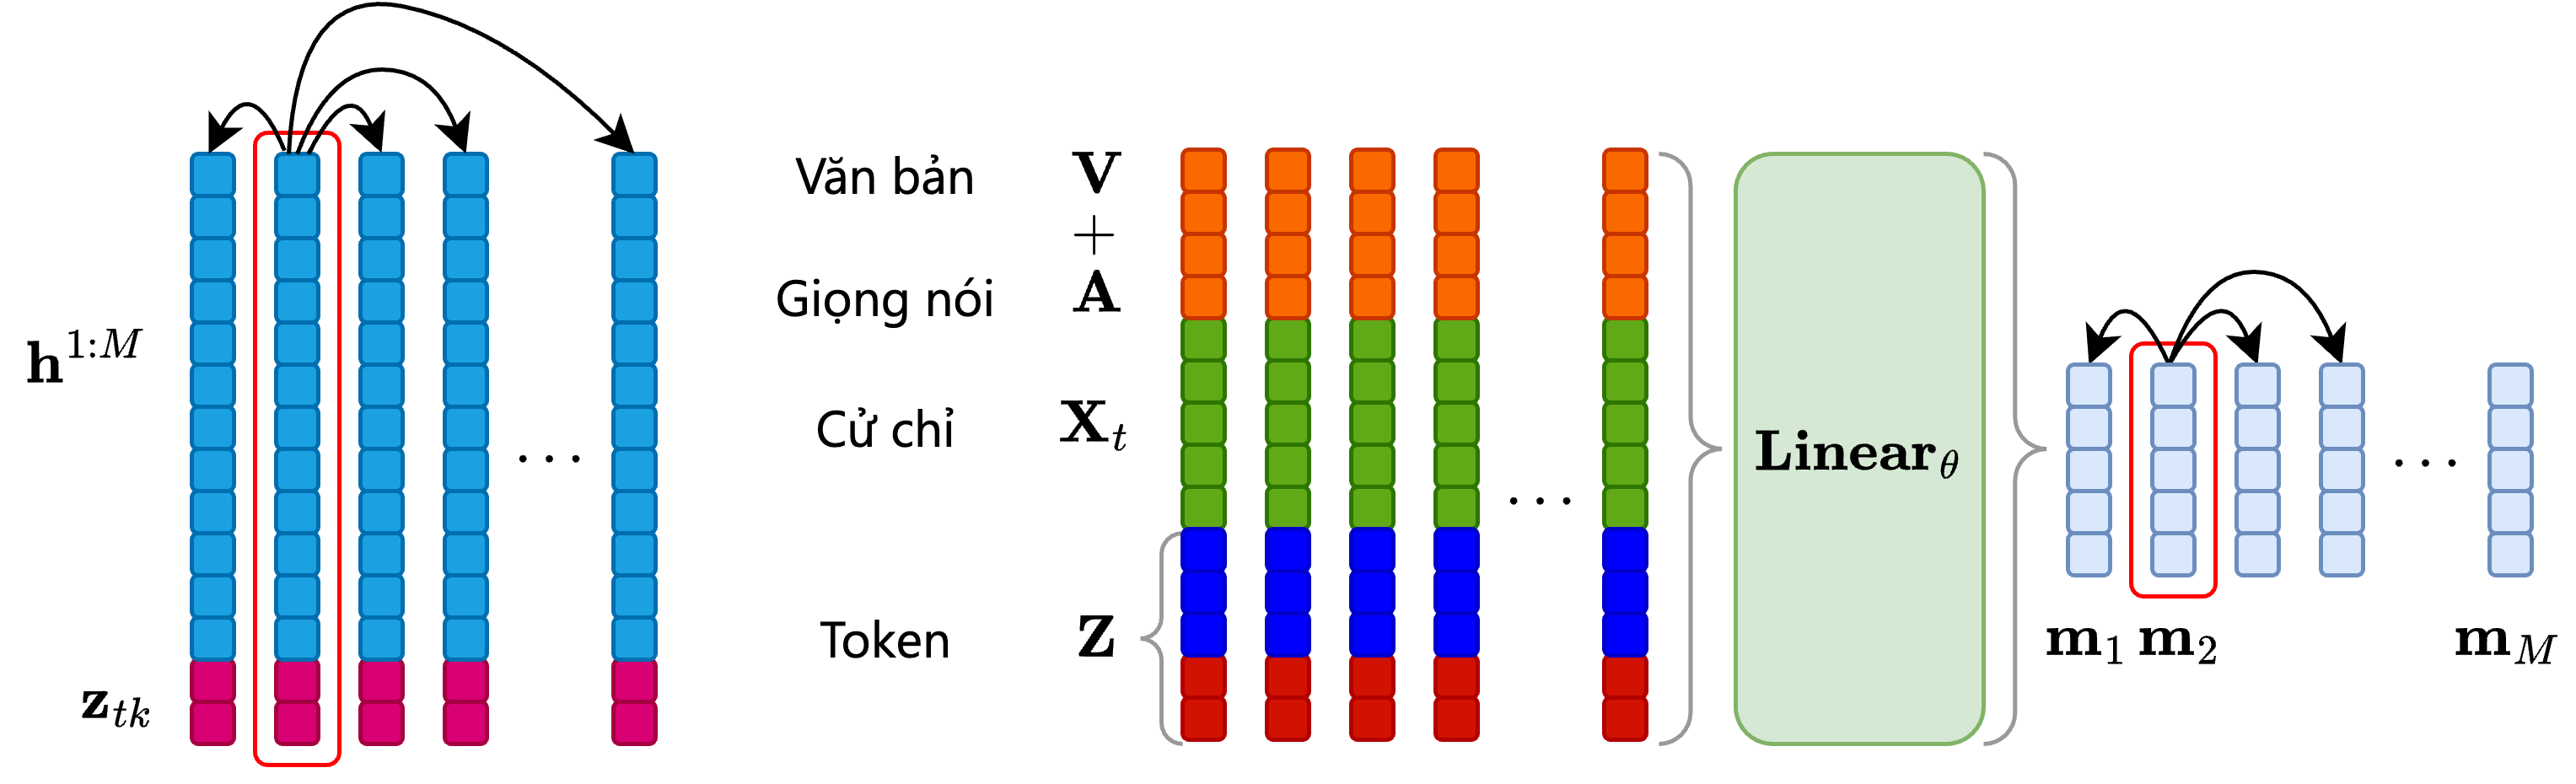
\includegraphics[width=0.7\textwidth]{CrossLocalAttention}
%	\end{figure}
	%	\textbf{Cross-Local Attention}
	%	\begin{equation*} \label{eq:attention}
		%		\operatorname{Attention}(\mathbf{Q}, \mathbf{K}, \mathbf{V}, \mathbf{M})=\operatorname{softmax}\left(\frac{\mathbf{Q} \mathbf{K}^{T}+\mathbf{M}}{\sqrt{C}}\right) \mathbf{V}
		%	\end{equation*}
	%	
	%
	\begin{columns}
		\begin{column}{0.5\textwidth}
				\begin{itemize}
					\item Concat cảm xúc $\mathbf{E}$ và cử chỉ khởi tạo $\mathbf{S}$ để được vector latent $\mathbf{Z} \in \mathbb{R}^{256}$
					\item Cộng vector $\mathbf{Z}$ với vector timestep $\mathbf{T}$ để được vector $\mathbf{Z}$ và replicate $\mathbf{Z}$ $M$ lần để được $\mathbf{Z} \in \mathbb{R}^{[1:M] \times 256}$
					\item Concat các đặc trưng âm thanh $\mathbf{A}$, văn bản $\mathbf{V}$, cử chỉ $\mathbf{x}_{t}$ và $\mathbf{Z}$ để được vector đặc trưng theo từng frame.
					\item Thực hiện Cross-Local Attention trên vector đặc trưng từng frame để được đặc trưng $\mathbf{h}^{[1:M]}$.
					\item Sử dụng $\mathbf{Z}$ làm $\texttt{CLS}$ token cho $\mathbf{h}^{[1:M]}$ trước khi đi qua Transformer Encoder.
				\end{itemize}
				
		\end{column}
		
		\begin{column}{0.5\textwidth}
		\begin{figure}
				\centering
				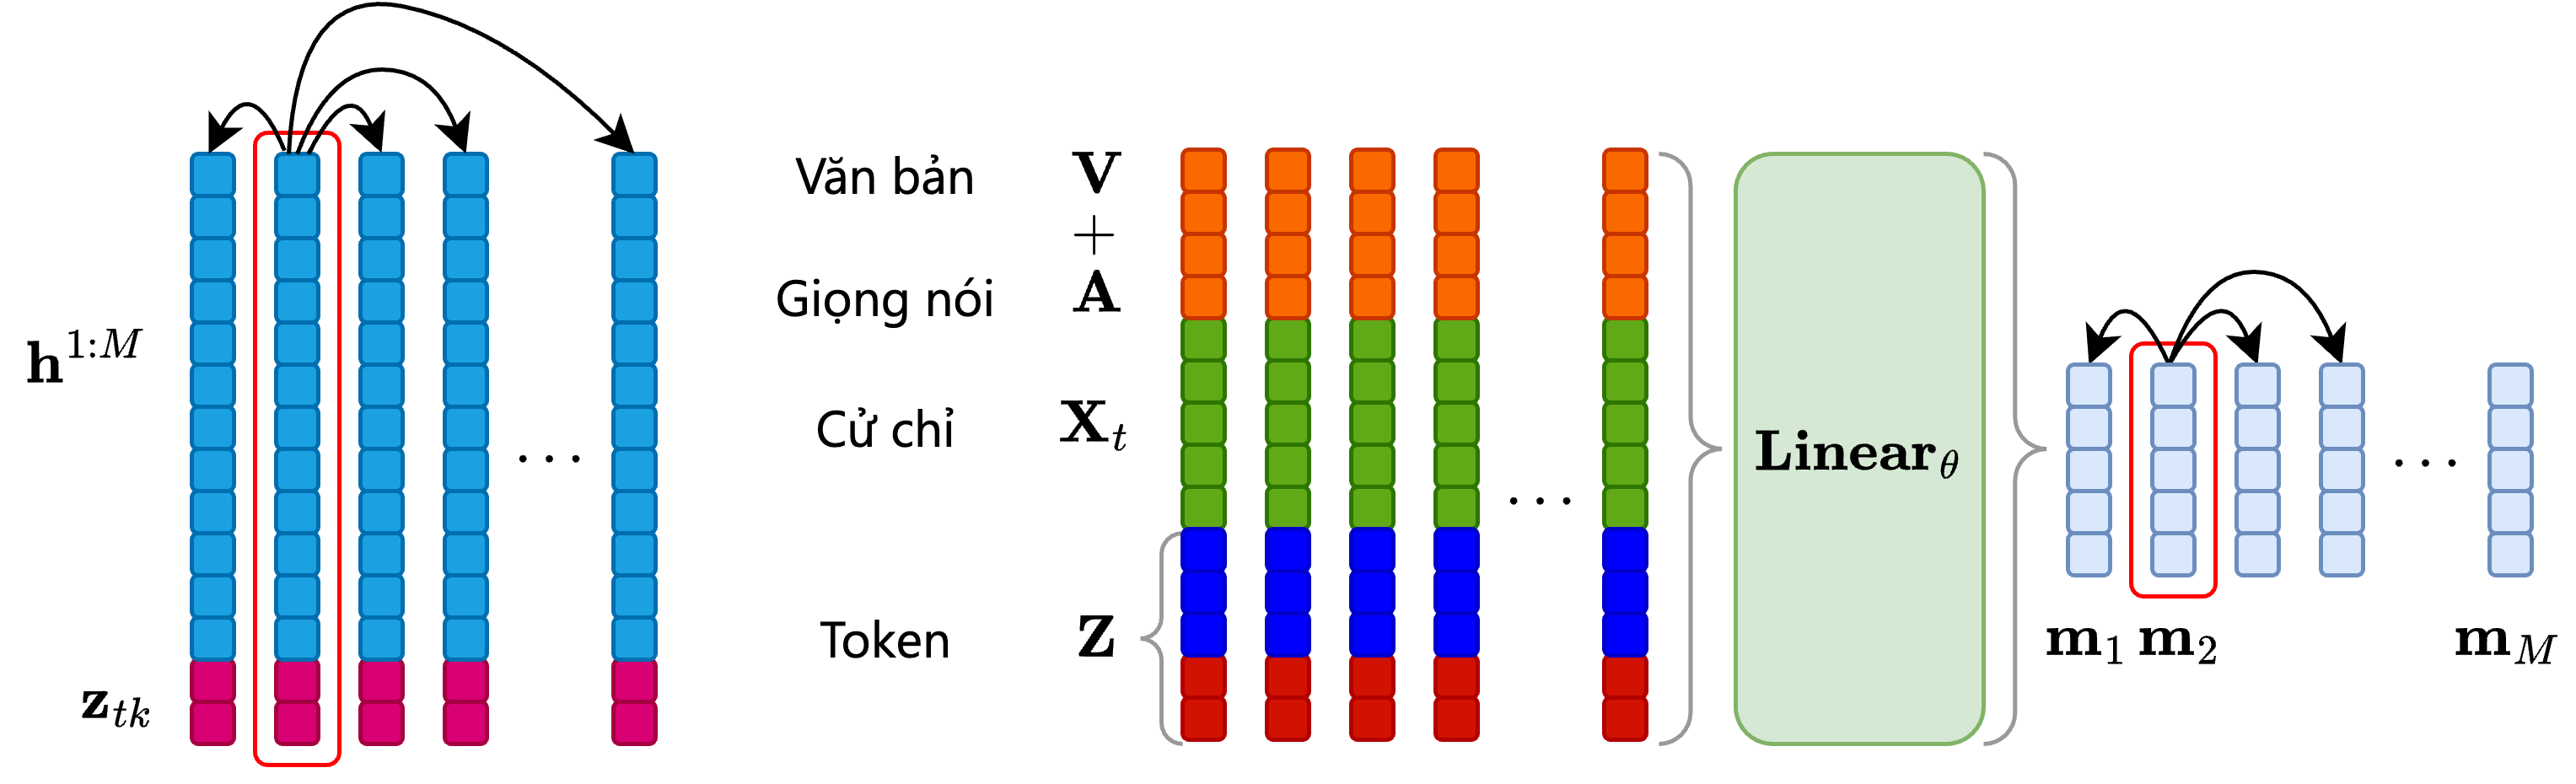
\includegraphics[width=\linewidth]{CrossLocalAttention}
			\end{figure}
	\end{column}
	\end{columns}
\end{frame}

\begin{frame}{Mô hình OHGesture}
	\begin{figure}
		\centering
		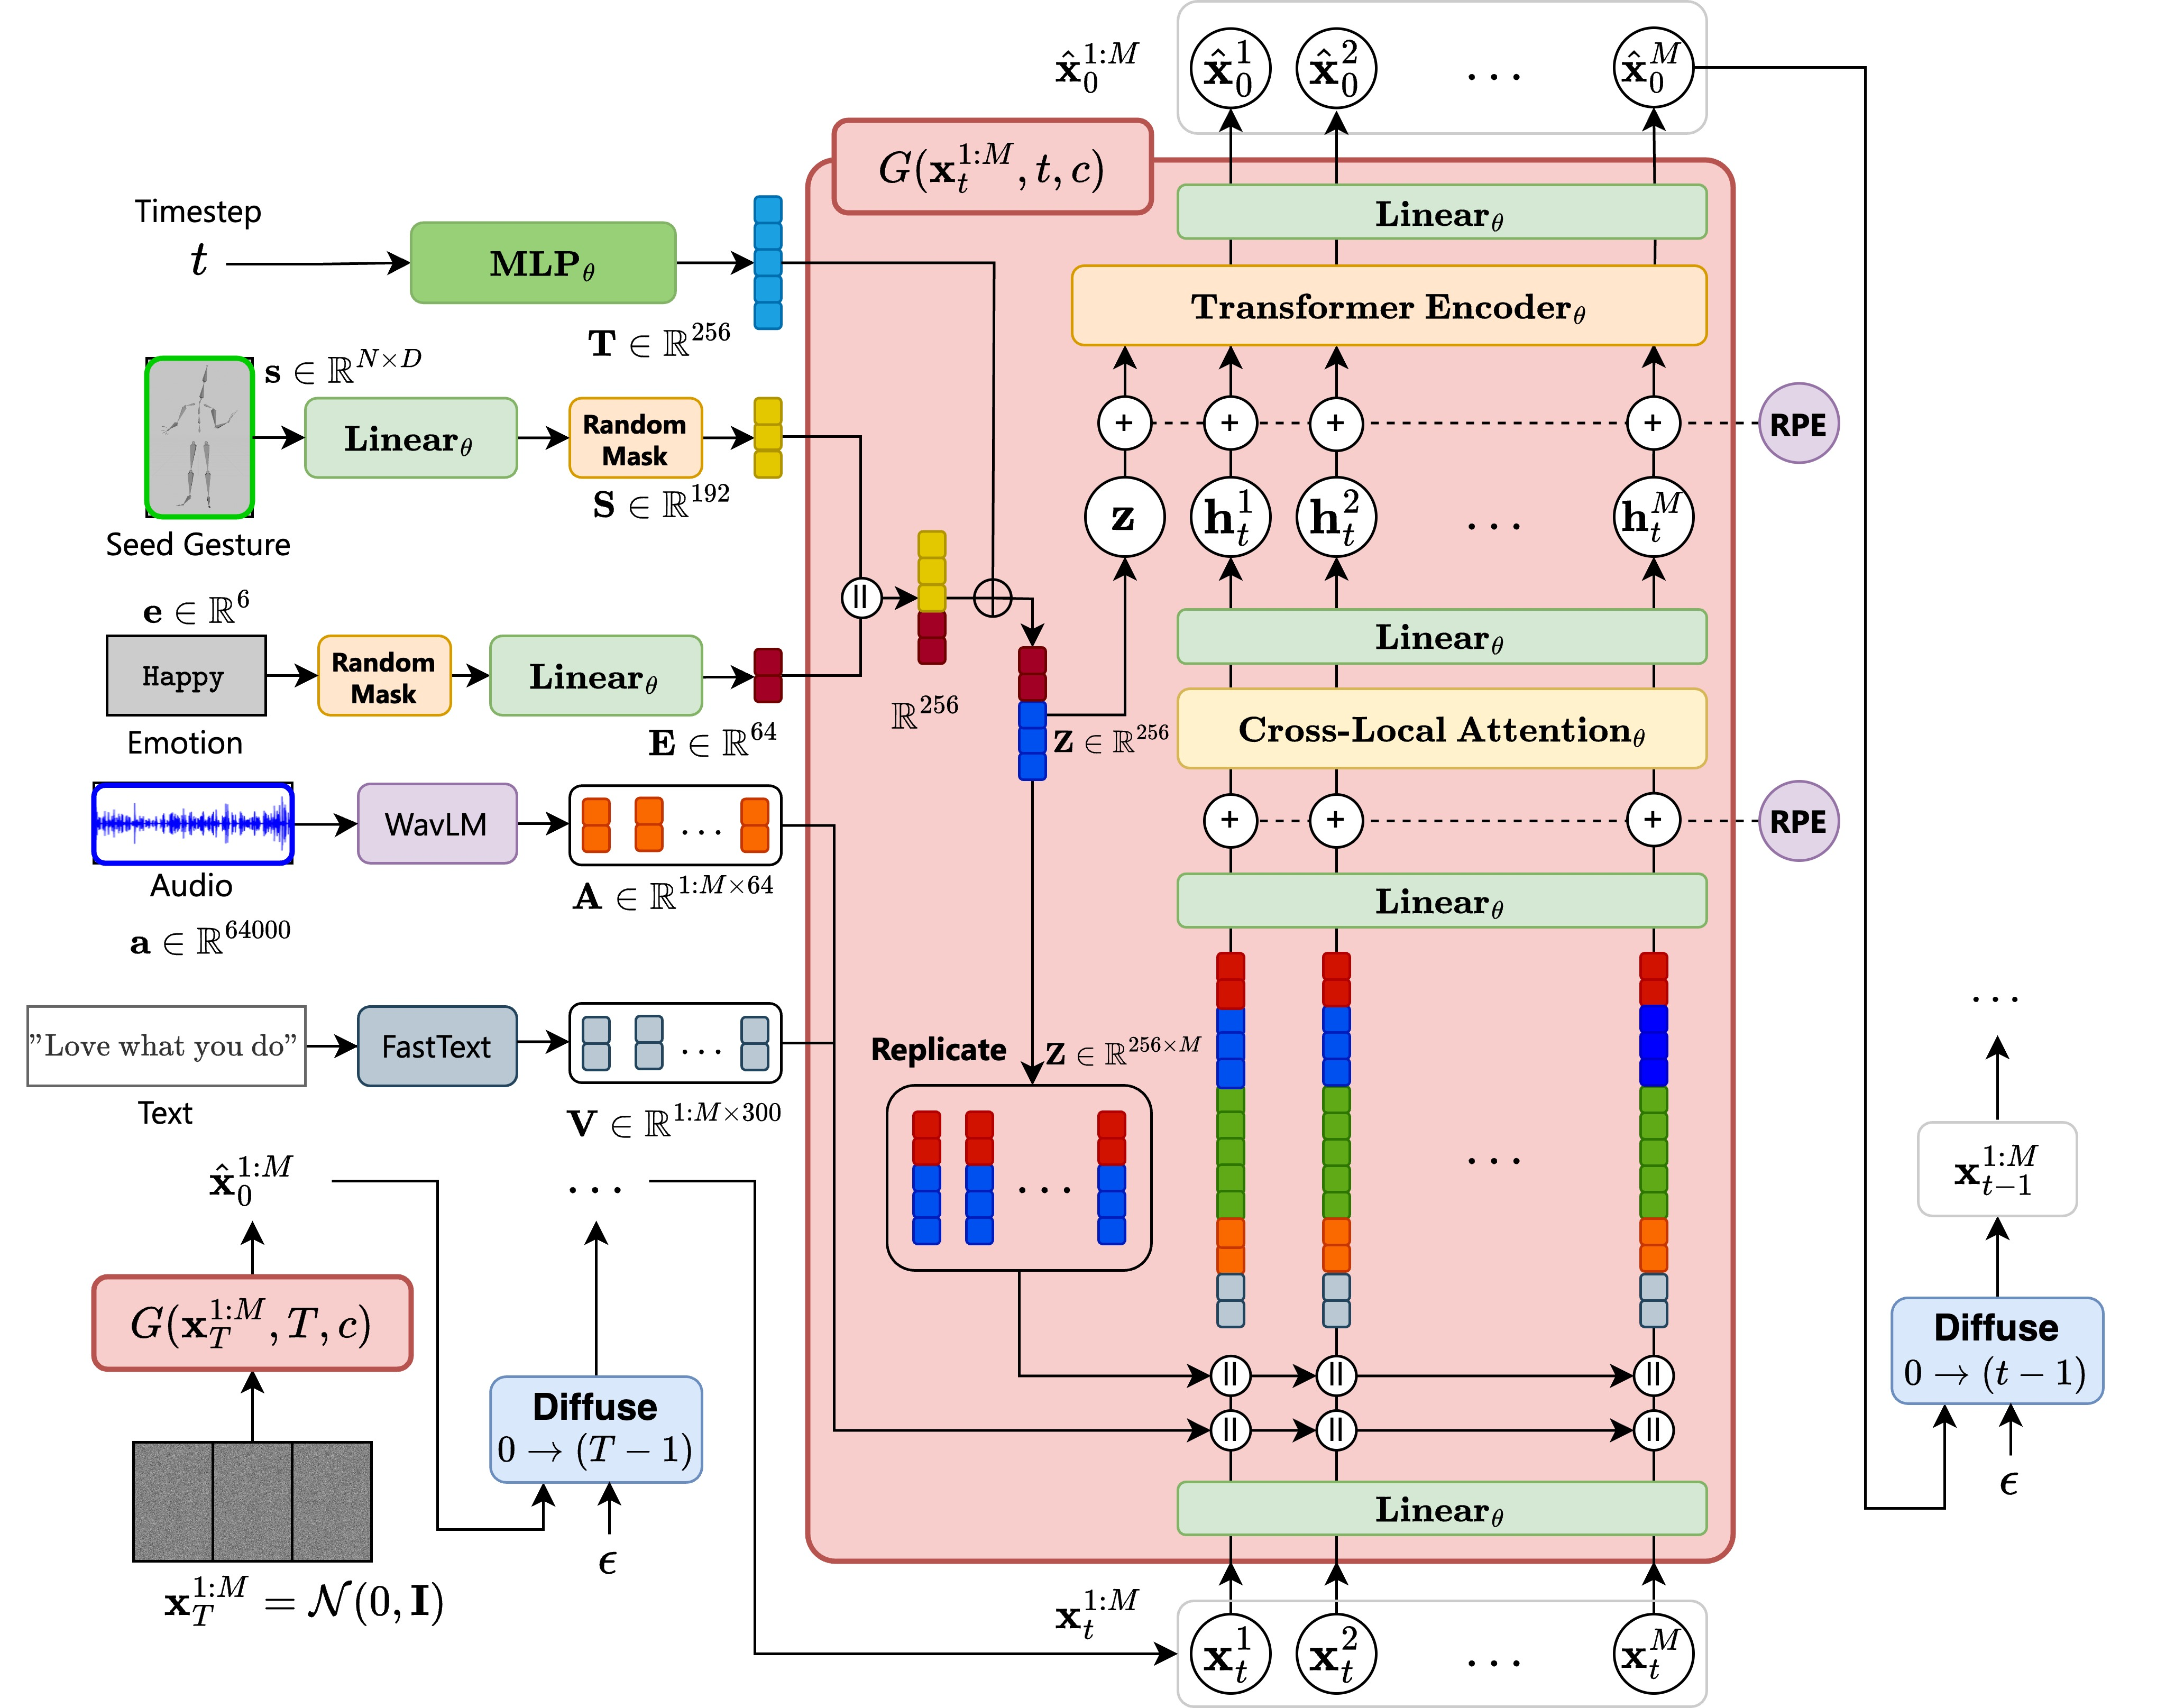
\includegraphics[width=0.9\linewidth]{OHGesture}
	\end{figure}
\end{frame}






\begin{frame}{Giải thích cơ chế Attention}
	\begin{figure}
		\centering
		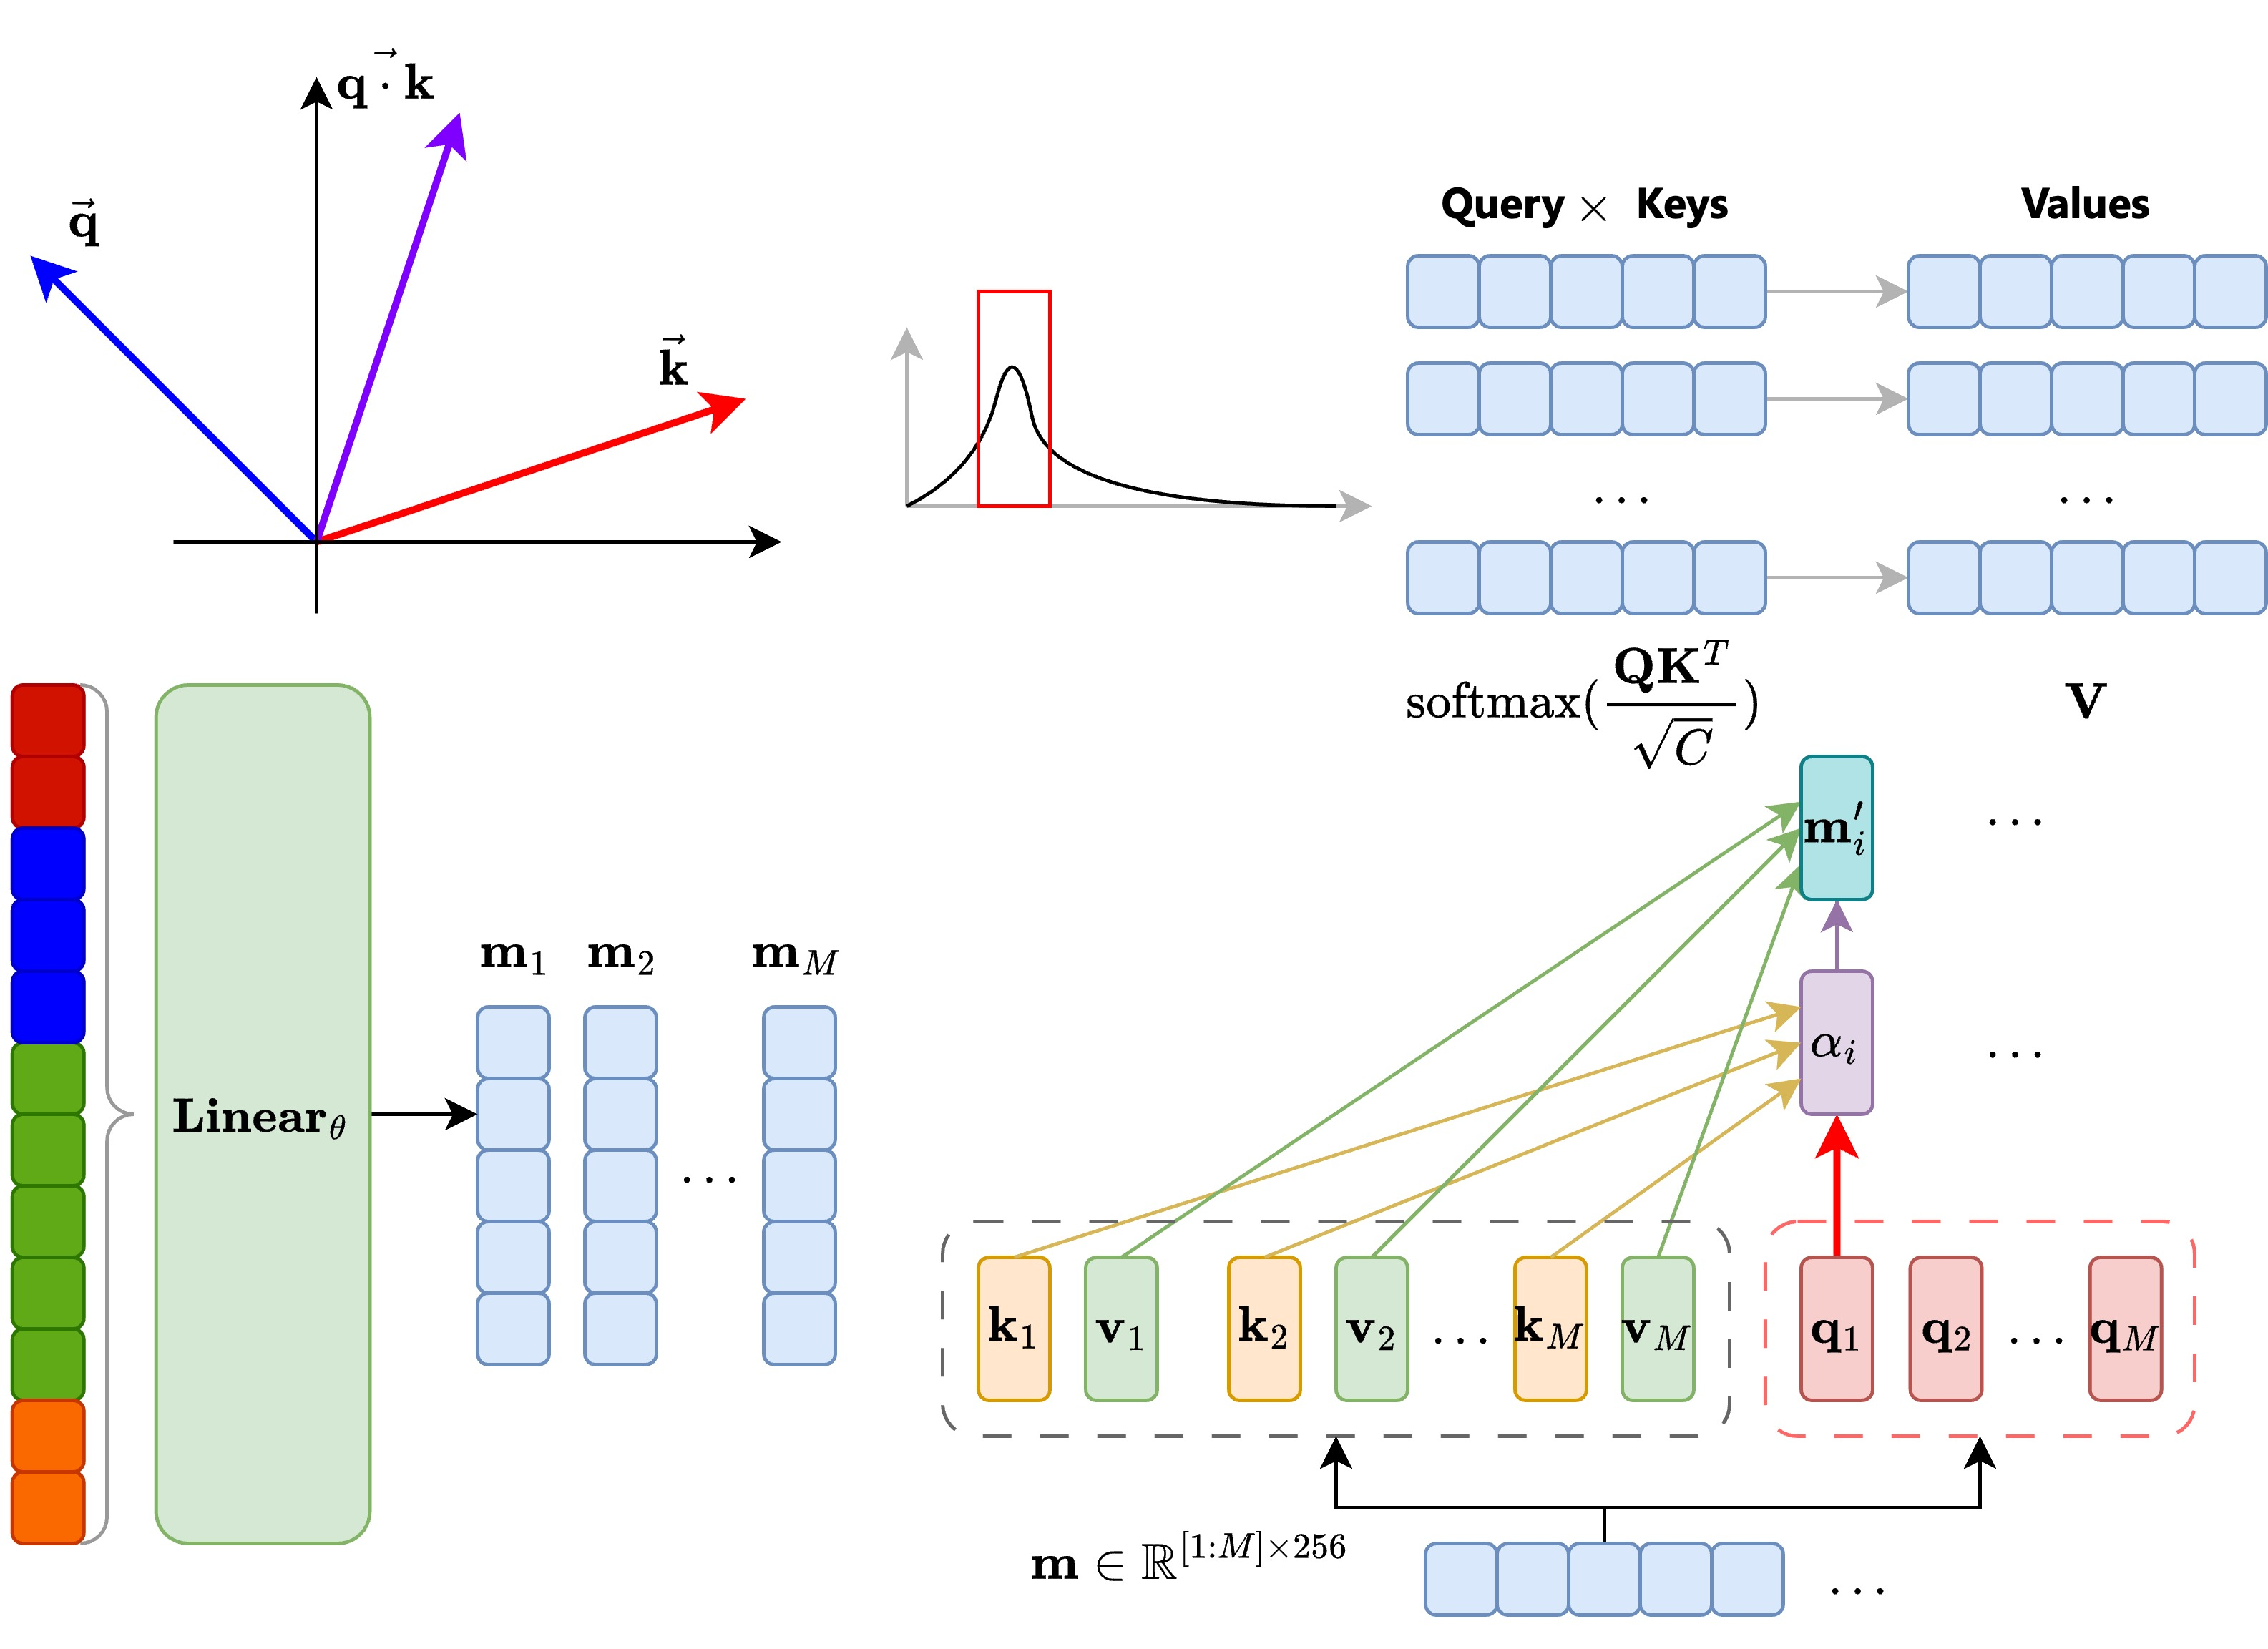
\includegraphics[width=0.85\linewidth]{Attention}
	\end{figure}
\end{frame}



%\begin{frame}
%	\begin{figure}
%		\centering
%		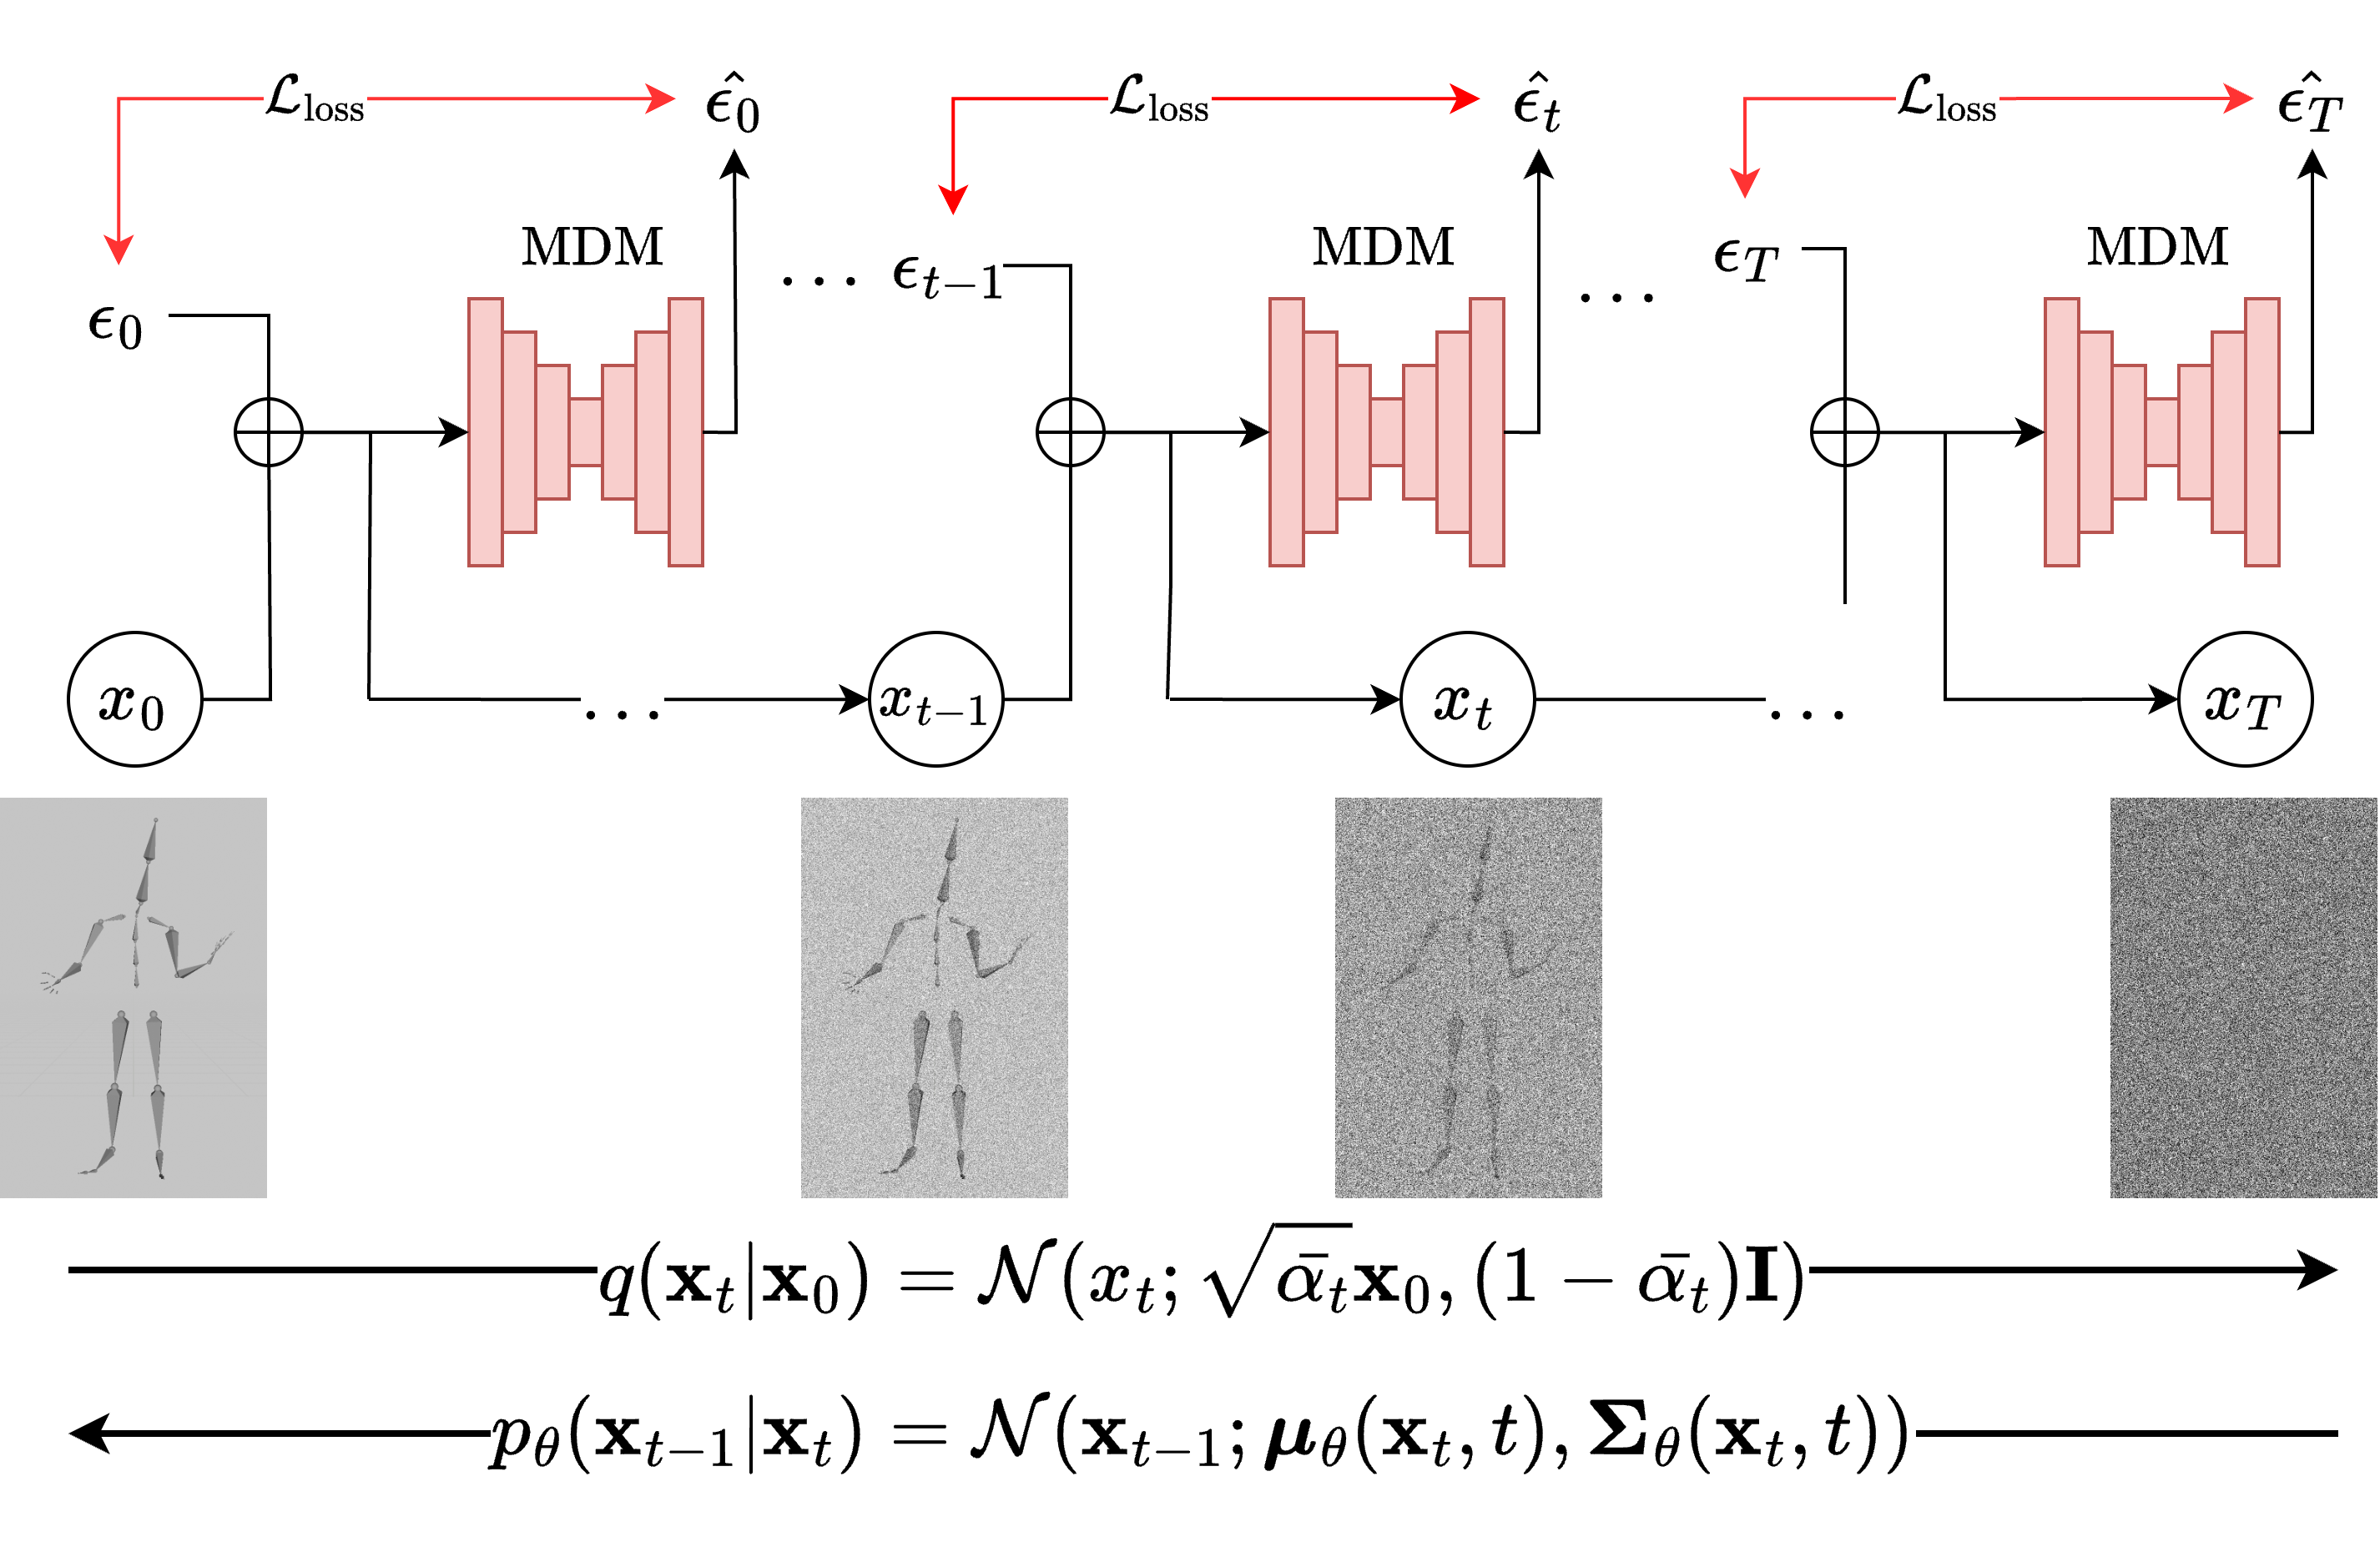
\includegraphics[width=0.8\linewidth]{DiffusionProcess}
%	\end{figure}
%\end{frame}


%\begin{figure} 
%	\centering
%	\includegraphics[width=0.8\linewidth]{DiffusionForward}
%\end{figure}


%\begin{frame}
%	
%	$
%	\label{Gaussian}
%	q\left(x_t \mid x_{t-1}\right)=\mathcal{N}\left(x_t ; \sqrt{1-\beta_t} x_{t-1}, \beta_t \mathbf{I}\right)
%	$
%	
%	$
%	\label{eq1}
%	q\left({x}_{1:T} \mid {x}_0\right)=\prod_{t=1}^T q\left({x}_t \mid {x}_{t-1}\right)
%	$
%	$
%	p_\theta\left({x}_{t-1} \mid {x}_t\right)=\mathcal{N}\left({x}_{t-1} ; {\mu}_\theta\left({x}_t, t\right), {\Sigma}_\theta\left({x}_t, t\right)\right)
%	$
%	
%	$
%	q\left({x}_t \mid {x}_0\right)=\mathcal{N}\left({x}_t ; \sqrt{\bar{\alpha}_t} {x}_0,\left(1-\bar{\alpha}_t\right) \mathbf{I}\right)
%	$
%	
%	$
%	\hat{x}_0=G\left(x_t, t, c\right)
%	$
%\end{frame}

	
%	\begin{columns}
	%		\begin{column}{0.5\textwidth}
		%			\textbf{DDPM (stochastic sampling):}
		%			\begin{itemize}
			%			\item Predict $x_0$ from $x_t$
			%			
			%			\item Convert to $\epsilon_{pred}$
			%			
			%			\item Use the formula:
			%			
			%			$$x_{t-1} = \frac{1}{\sqrt{\alpha_t}} x_t - \frac{1-\alpha_t}{\sqrt{1-\bar{\alpha}t}\sqrt{\alpha_t}} \epsilon_{\text{pred}} + \sigma_t z$$
			%			
			%			\item where $z \sim \mathcal{N}(0,I)$ is random noise
			%			\end{itemize}
		%			
		%		\end{column}
	%		
	%		\begin{column}{0.5\textwidth}
		%			\textbf{DDIM (deterministic sampling):}
		%			
		%			Predict $x_0$ from $x_t$
		%			
		%			NO additional noise term ($\sigma_t = 0$)
		%			
		%			Use the formula:
		%			
		%			$x_{t-1} = \sqrt{\bar{\alpha}{t-1}} x_0^{\text{pred}} + \sqrt{1-\bar{\alpha}_{t-1}} \epsilon_{\text{pred}}$
		%			
		%			Where:
		%			\begin{itemize}
			%			\item $\bar{\alpha}_t$ is the cumulative product of $\alpha$'s from 1 to t
			%			\item $\epsilon_{pred}$ is derived from $x_0$ prediction using:
			%			\item $\epsilon_{pred} = \frac{x_t - \sqrt{\alpha_t}x_{0_{pred}}}{\sqrt{1-\alpha_t}}$
			%			\end{itemize}
		%		\end{column}
	%	\end{columns}
	
